%
% tikztemplate.tex -- Template für standalone TIKZ Bilder
%
% (c) 2019 Prof Dr Andreas Müller, Hochschule Rapperswil
%
\documentclass[tikz,12pt]{standalone}
\usepackage{amsmath}
\usepackage{times}
\usepackage{txfonts}
\usepackage{pgfplots}
\usepackage{csvsimple}
\usetikzlibrary{arrows,intersections,math}
\begin{document}
\begin{tikzpicture}[>=latex]

% hier Bild-Definition einfüllen
\node at (0,0) {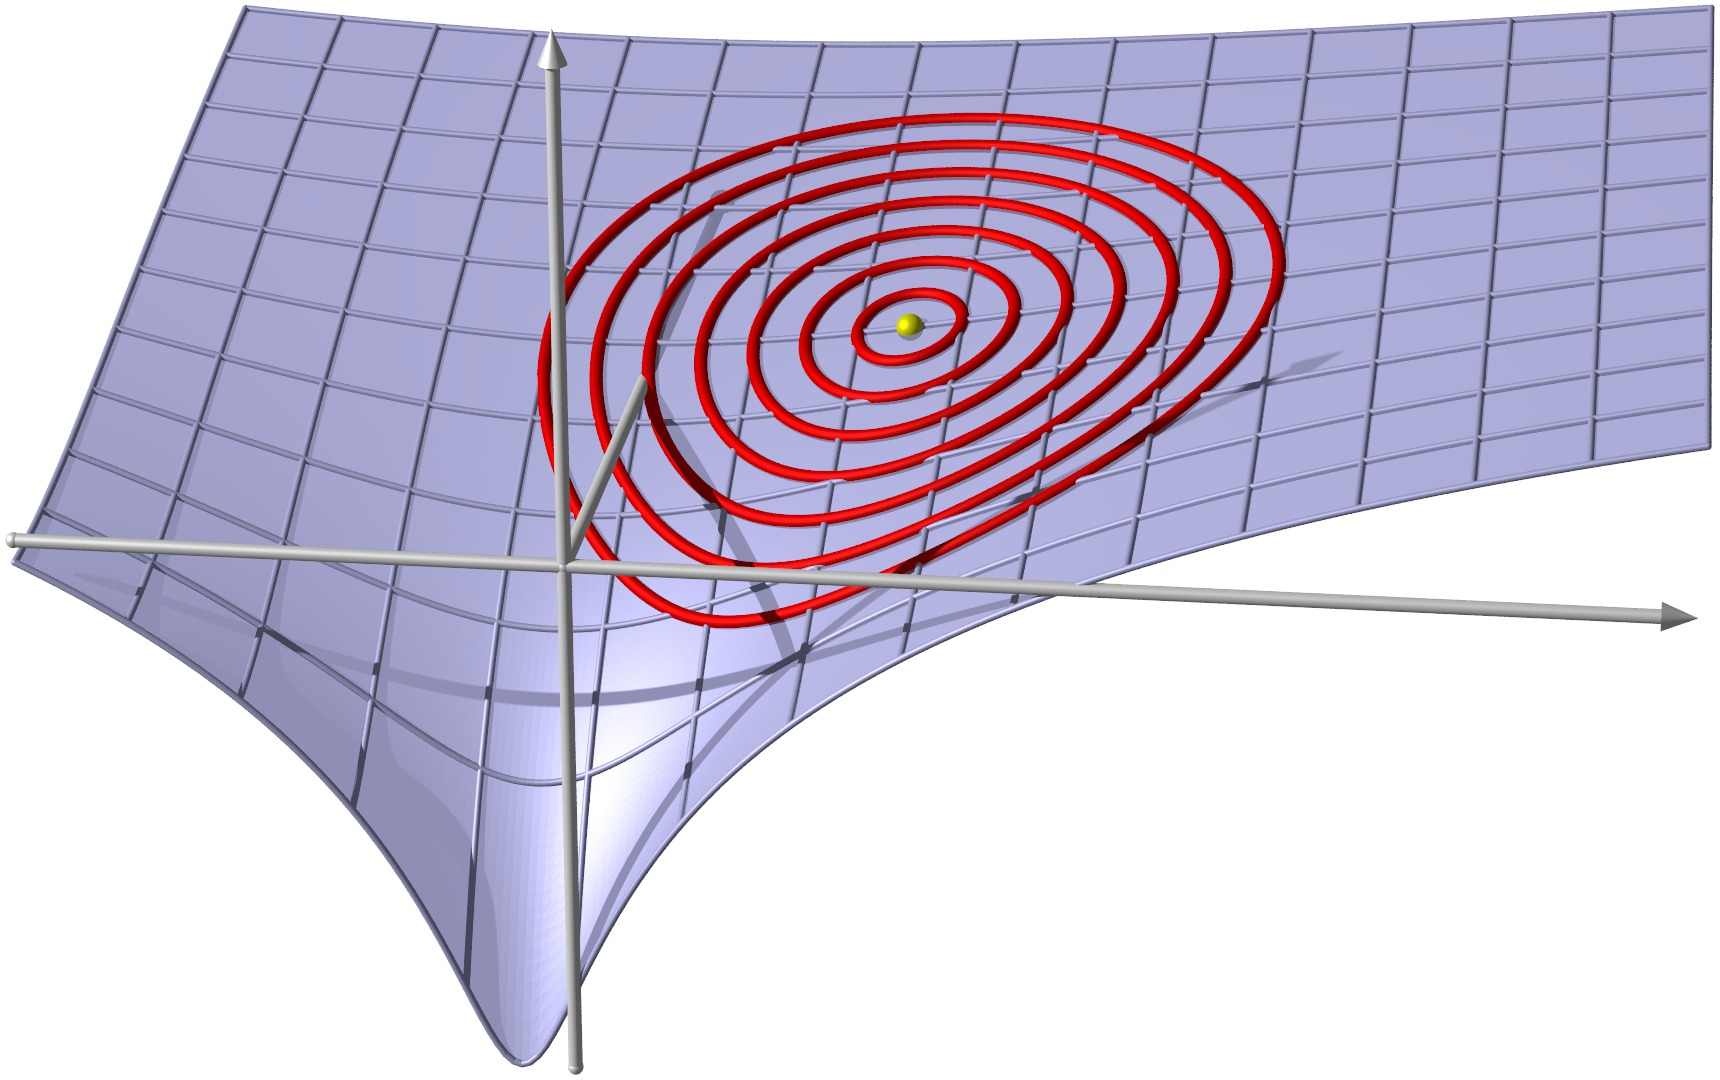
\includegraphics[width=12cm]{meanvalue.jpg}};
\node at (5.9,-0.3) {$x$};
\node at (-2.0,3.7) {$z$};
\node[color=white] at (0.5,1.8) {$C$};

\end{tikzpicture}
\end{document}

